\documentclass[conference]{IEEEtran}
\usepackage[utf8]{inputenc}
\usepackage[spanish]{babel}
\usepackage{graphicx}
\usepackage{amsmath}
\usepackage{cite}
\usepackage{hyperref}
\usepackage{subcaption} % Vital para las figuras con literales

\begin{document}

\title{Densidad Espectral de Potencia (PSD) de Señales Aleatorias en GNU Radio}

\author{

\IEEEauthorblockN{juan david camacho gonzalez (Cód: 2210428), Valentina Arguellez Angulo (Cód: 2215670)}
\IEEEauthorblockA{\textit{Escuela de Ingenierías Eléctrica, Electrónica y de Telecomunicaciones} \\
\textit{Universidad Industrial de Santander}\\
Bucaramanga, Colombia \\
juan2210428@correo.uis.edu.co \\
Valentina2215670@correo.uis.edu.co\\}
\vspace{0.2cm}
\textit{Repositorio GitHub:} \url{https://github.com/singeku/ComII_G2_equipo2/tree/practica_2}
}

\maketitle

% --- Aquí se ensamblan los módulos que hará cada integrante ---
\begin{abstract}
This document presents the comprehensive analysis of the Power Spectral Density (PSD) of random signals and real-world data using the GNU Radio software environment. The methodology focuses on the transmission of random bit streams, compressed images (.jpg), and raw audio (.wav) to evaluate their spectral behavior, demonstrating the emergence of Direct Current (DC) components and harmonic frequencies due to data redundancy. Furthermore, the physical and mathematical impact of the Samples per Symbol (Sps) parameter is evaluated, proving that time-scaling increases the energy per bit without altering the physical bandwidth of the information. Finally, the interpolating FIR filter coefficients are modified to implement and analyze diverse line codes (NRZ, RZ, Manchester) and digital modulations (OOK, BPSK, ASK, Sinc, Raised Cosine). Spectral analysis verifies how each specific waveform reshapes the spectral envelope, successfully eliminating the DC component in Manchester coding and maximizing spectral efficiency by suppressing infinite side lobes through the Raised Cosine filter.
\end{abstract}

\begin{IEEEkeywords}
Amplitude Shift Keying, GNU Radio, Line Coding, Phase Shift Keying, Power Spectral Density, White Noise.
\end{IEEEkeywords}
\section{Introducción}

La densidad espectral de potencia (PSD) es una herramienta fundamental para analizar cómo se distribuye la potencia de una señal en frecuencia, lo cual permite evaluar ancho de banda, componente DC y ocupación espectral en sistemas de comunicaciones digitales \cite{ortega_reyes,proakis}. En señales aleatorias binarias, la PSD depende tanto de la estadística de la fuente como de la forma del pulso empleado en la transmisión.

En esta práctica se estudió la PSD de señales binarias aleatorias en GNU Radio Companion, considerando distintos valores de muestras por símbolo (\textit{Sps}), ruido blanco y fuentes reales obtenidas a partir de archivos de imagen y audio \cite{guia_lab3,gnuradio}. Además, se analizaron modificaciones en la codificación de línea y en la conformación de pulso para identificar su efecto sobre la componente DC y la distribución espectral de la señal.
\section{Metodología}

La práctica se desarrolló en GNU Radio Companion a partir del flujograma base suministrado en la guía del laboratorio \cite{guia_lab3,gnuradio}. El procedimiento se dividió en cuatro etapas.

\subsection{Señal binaria aleatoria bipolar}
Se generó una secuencia binaria aleatoria y se convirtió de unipolar a bipolar para reducir la componente DC. Luego se aplicó un bloque \textit{Interpolation FIR Filter} y se evaluaron los casos \(Sps=1\), \(4\), \(8\) y \(16\), registrando la forma temporal, la PSD y los parámetros \(R_b\), \(F_s\) y ancho de banda.

\subsection{Caracterización de ruido blanco}
Se configuraron las fuentes virtuales en los puntos \(p4\) y \(p5\) para observar el ruido blanco en el dominio del tiempo y en frecuencia. Además, se comparó el efecto de variar la amplitud del generador sobre el nivel de potencia espectral.

\subsection{Análisis con fuentes reales}
Se reemplazó el bloque \texttt{Random Source} por una cadena formada por \texttt{File Source}, \texttt{Unpack K Bits} y \texttt{Char to Float}, usando como entradas los archivos \texttt{rana.jpg} y \texttt{sonido.wav}. Con ello se comparó la PSD de fuentes reales frente a la de una fuente aleatoria ideal.

\subsection{Preguntas de control}
Finalmente, se modificó el vector de coeficientes \(h\) del filtro interpolador para evaluar cambios en codificación de línea y conformación de pulso, respondiendo de forma sintética las preguntas de control del laboratorio.
\section{Resultados y Discusión}

% --- Módulo del Punto 2 (A cargo del Integrante A) ---
%\input{modulos/resultados/01_punto2}

% --- Módulo del Punto 3 (A CARGO TUYO: Ruido AWGN) ---
\FloatBarrier
\subsection{Señal binaria aleatoria bipolar con diferentes valores de \(Sps\)}

Se analizó la densidad espectral de potencia (PSD) de una señal binaria aleatoria bipolar para distintos valores de muestras por símbolo (\(Sps = 1, 4, 8, 16\)). La Tabla \ref{tab:parametros_sps} resume los parámetros principales y el comportamiento temporal y espectral observado en cada caso. La Figura \ref{fig:sps_signal} presenta los resultados para \(Sps=1\), \(4\), \(8\) y \(16\), identificados individualmente en las subfiguras \ref{fig:sps1}--\ref{fig:sps16}.

En todos los ensayos se mantuvo constante la tasa de bits \(R_b\), mientras que la frecuencia de muestreo \(F_s\) aumentó proporcionalmente con \(Sps\). Por esta razón, el ancho de banda fundamental permaneció aproximadamente constante, aunque la representación temporal de la señal se hizo más detallada a medida que aumentó el sobremuestreo.

\begin{table}[H]
\caption{Comparación de la señal para diferentes valores de \(Sps\).}
\label{tab:parametros_sps}
\centering
\vspace{1mm}
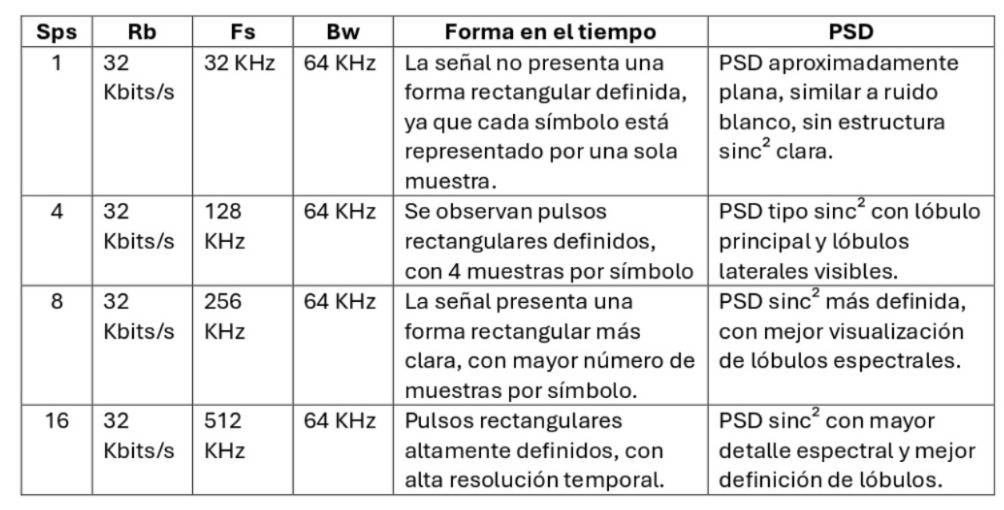
\includegraphics[width=0.95\columnwidth, trim=8 8 8 8, clip]{imagenes/tab.jpeg}
\vspace{-2mm}
\end{table}

\begin{figure}[H]
\centering
\begin{subfigure}[b]{0.48\columnwidth}
    \centering
    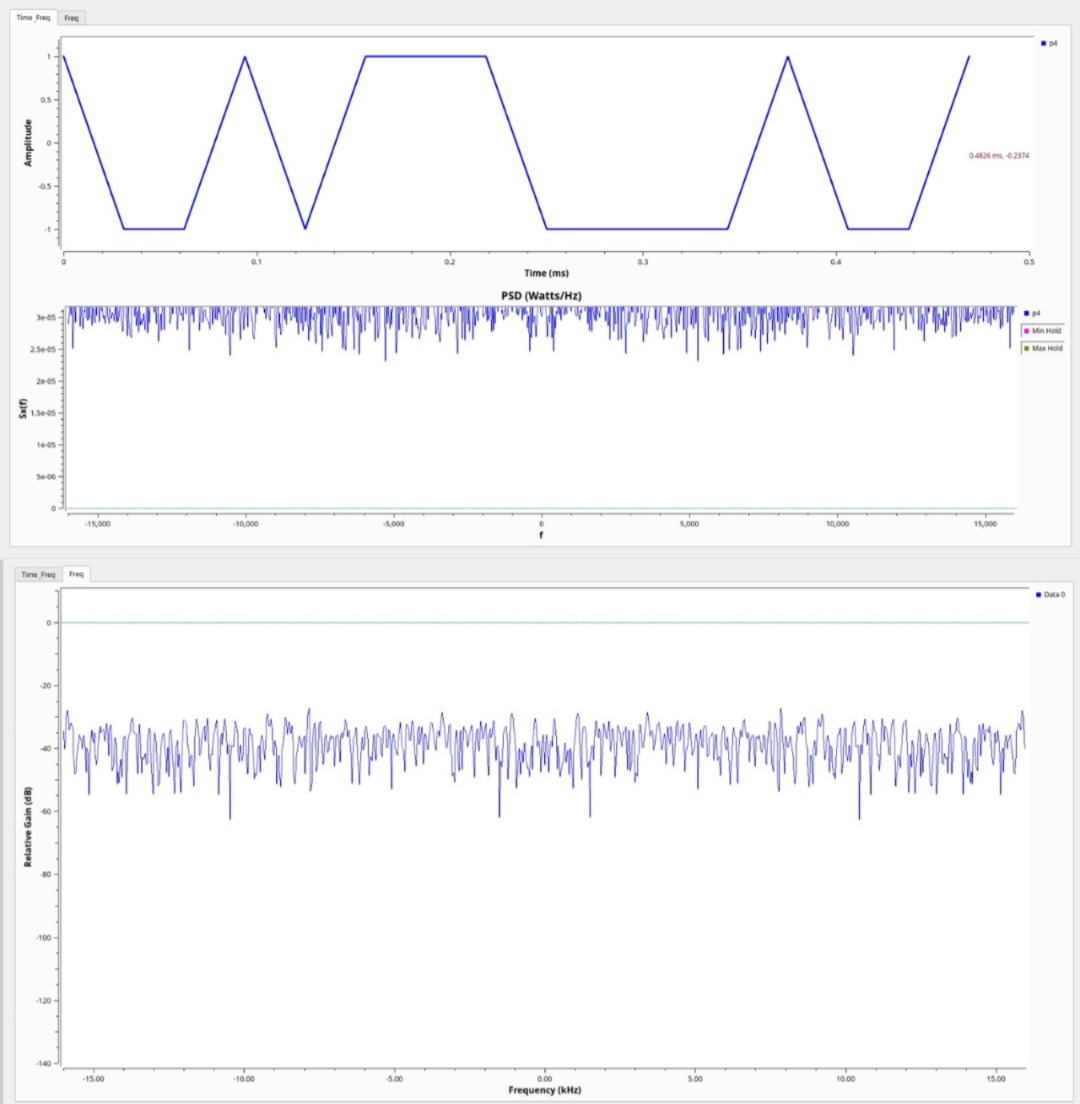
\includegraphics[width=\linewidth]{imagenes/Sps1.jpeg}
    \caption{\(Sps=1\)}
    \label{fig:sps1}
\end{subfigure}
\hfill
\begin{subfigure}[b]{0.48\columnwidth}
    \centering
    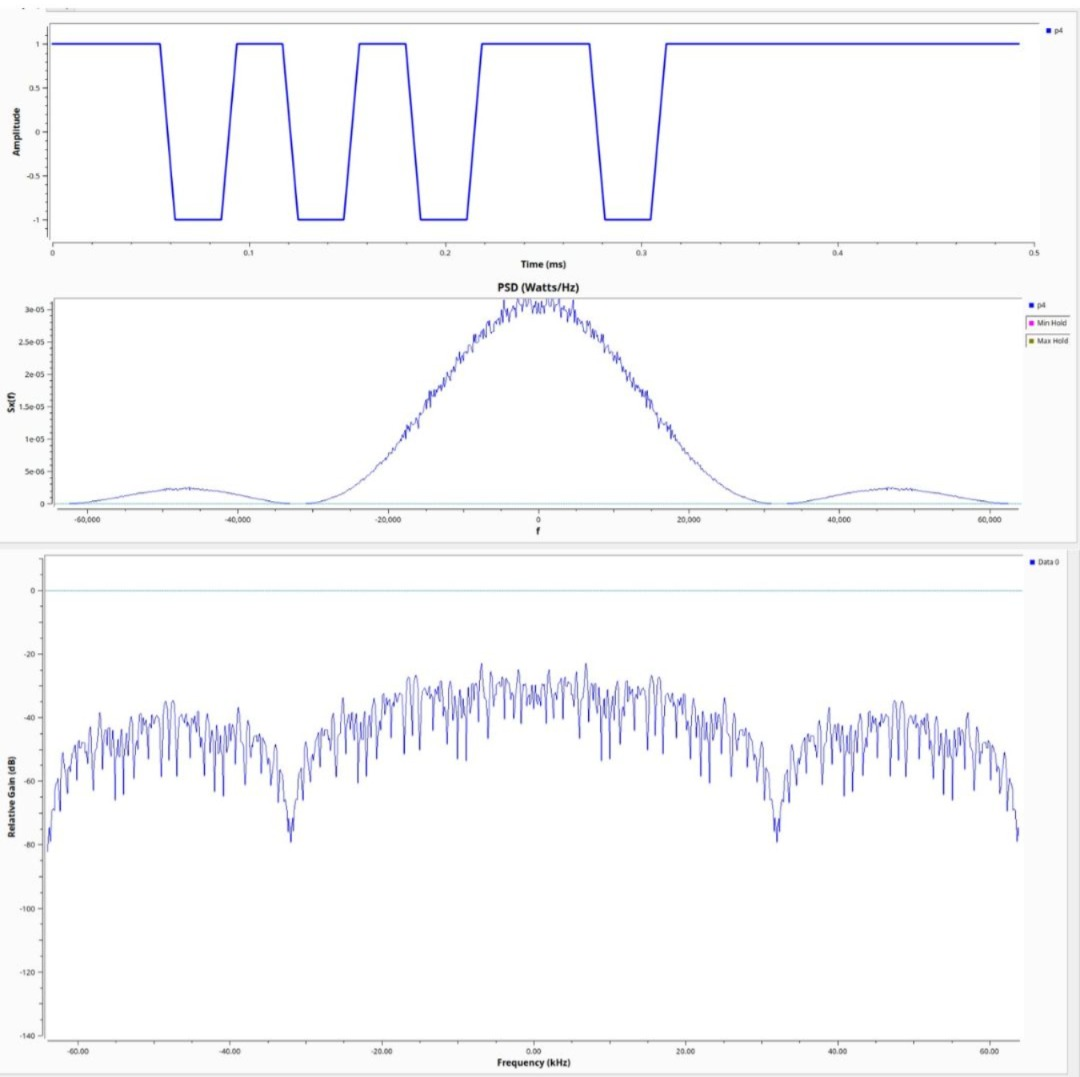
\includegraphics[width=\linewidth]{imagenes/Sps4.jpeg}
    \caption{\(Sps=4\)}
    \label{fig:sps4}
\end{subfigure}

\vspace{0.1cm}

\begin{subfigure}[b]{0.48\columnwidth}
    \centering
    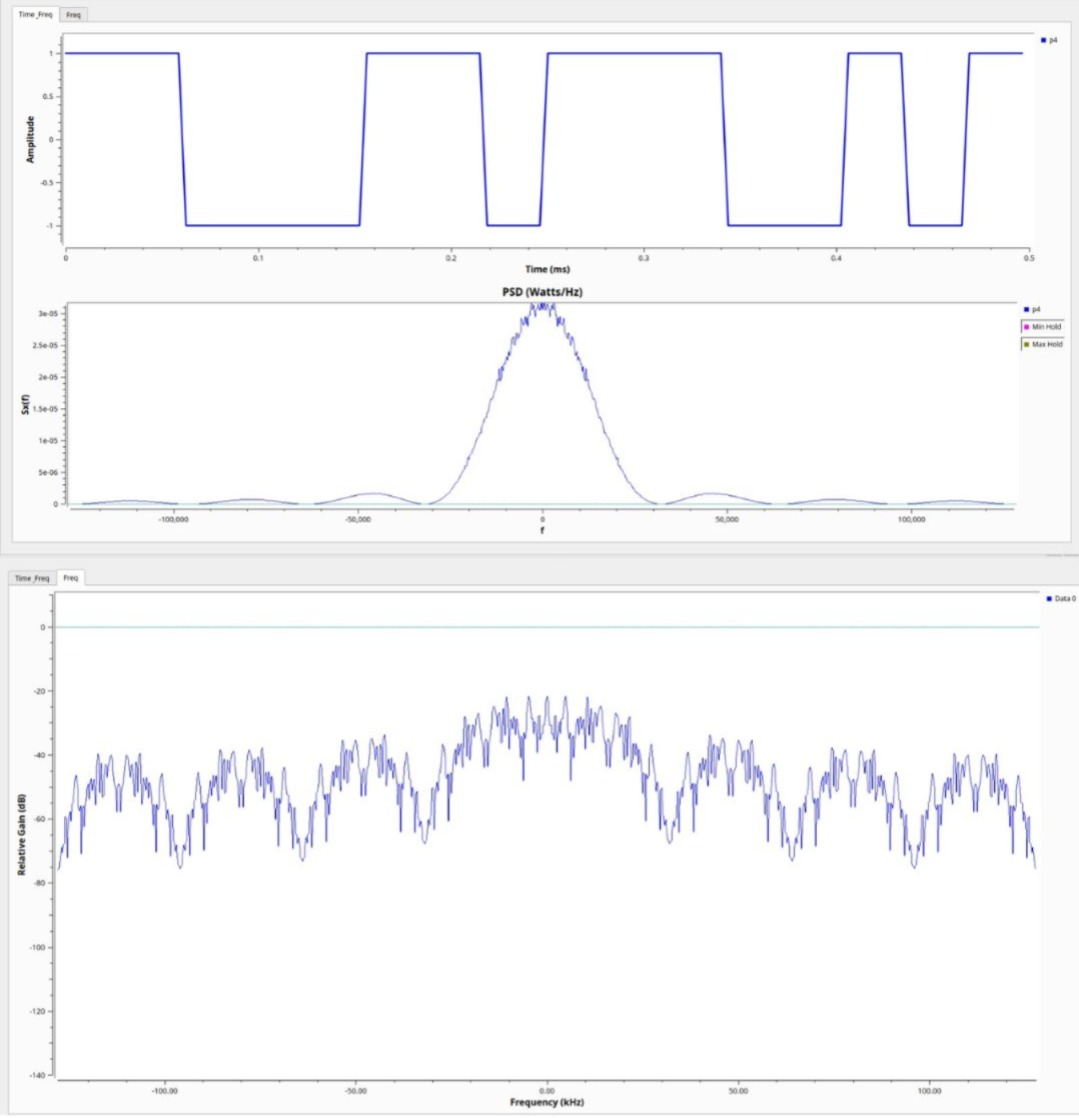
\includegraphics[width=\linewidth]{imagenes/Sps8.jpeg}
    \caption{\(Sps=8\)}
    \label{fig:sps8}
\end{subfigure}
\hfill
\begin{subfigure}[b]{0.48\columnwidth}
    \centering
    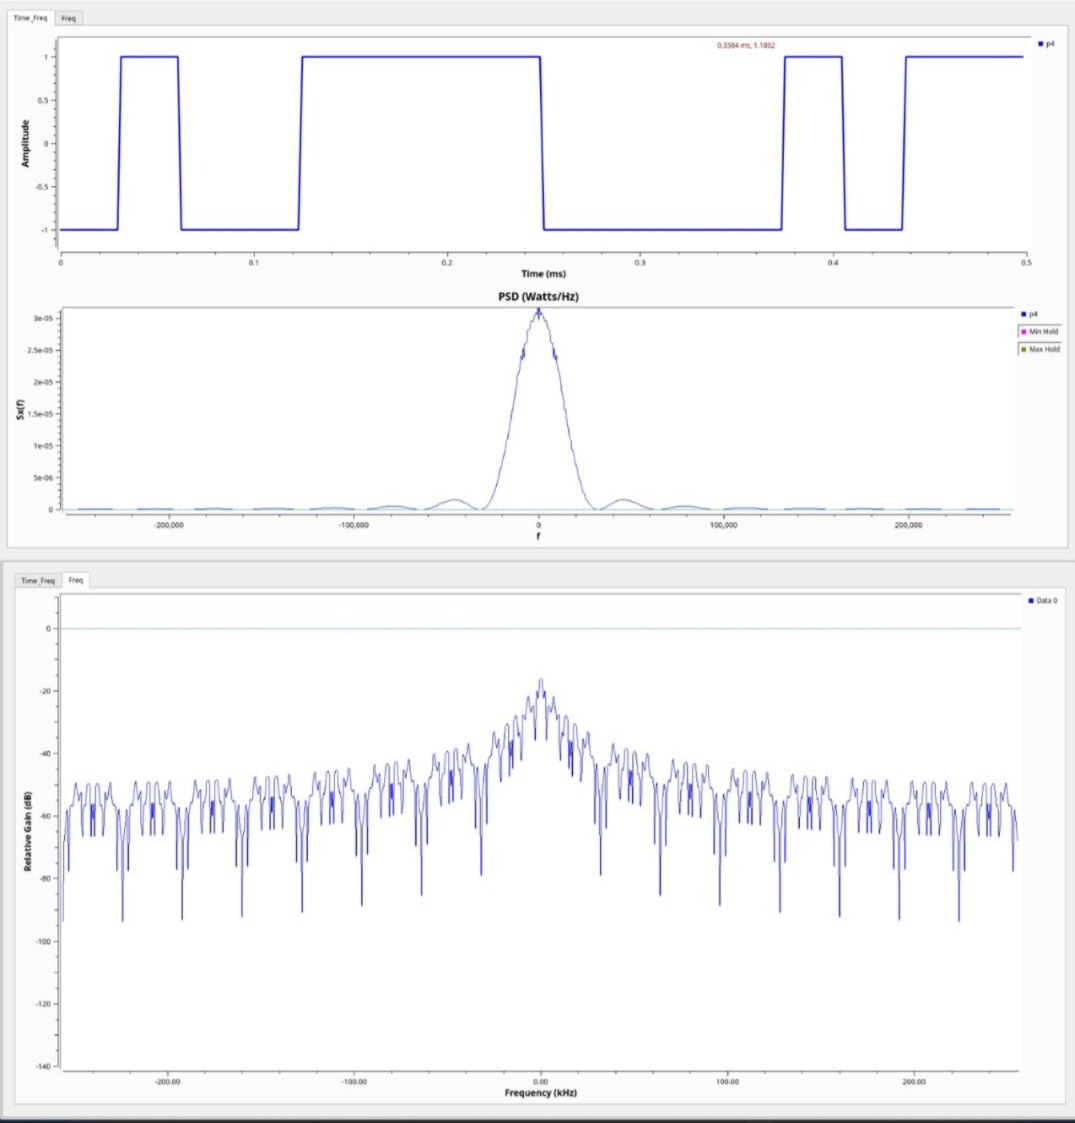
\includegraphics[width=\linewidth]{imagenes/Sps16.jpeg}
    \caption{\(Sps=16\)}
    \label{fig:sps16}
\end{subfigure}

\caption{Representación temporal y PSD de la señal binaria aleatoria bipolar para diferentes valores de \(Sps\).}
\label{fig:sps_signal}
\end{figure}

En la subfigura \ref{fig:sps1}, correspondiente a \(Sps=1\), cada símbolo queda representado por una sola muestra, por lo que la señal no exhibe una forma rectangular claramente definida y su PSD se aproxima a una distribución casi plana. En la subfigura \ref{fig:sps4}, para \(Sps=4\), ya se observan pulsos rectangulares distinguibles y aparece con mayor claridad la envolvente espectral tipo sinc\(^2\), con lóbulo principal y lóbulos laterales visibles.

En las subfiguras \ref{fig:sps8} y \ref{fig:sps16}, la forma temporal se observa con mayor resolución y la PSD presenta una definición espectral más clara. Sin embargo, el incremento de \(Sps\) no modifica la estructura espectral fundamental de la señal, sino que mejora su representación temporal y la visualización de sus componentes en frecuencia.

En consecuencia, el sobremuestreo facilita el análisis visual de la señal sin alterar la relación principal entre tasa de bits y ocupación espectral.
\FloatBarrier
% --- INICIO DEL MÓDULO: 02_punto3.tex ---

\subsection{Caracterización del Ruido Blanco en Tiempo y Frecuencia}

Al observar la señal en el dominio del tiempo, se evidenció una forma de onda erratica y sin ningún patrón repetitivo. Los picos de voltaje varían de forma impredecible en cada instante de muestreo, lo cual comprueba físicamente que las muestras de ruido blanco son variables aleatorias descorrelacionadas e independientes entre sí.

El fenómeno más destacable se registró en el dominio de la frecuencia. Al analizar la Densidad Espectral de Potencia (PSD), la gráfica no mostró lóbulos ni campanas (como ocurre con los pulsos rectangulares), sino que exhibió una banda completamente plana y horizontal que se extiende a lo largo de todo el rango de frecuencias observable por el analizador (desde $-f_s/2$ hasta $+f_s/2$). Esta "planitud" espectral es una característica del ruido blanco, demostrando que su energía se distribuye equitativamente en todas las frecuencias del espectro evaluado.

Al realizar pruebas variando el parámetro de amplitud del ruido en el bloque generador, se observó que la forma plana de la PSD no se altera. El único efecto visible en el espectro es un desplazamiento vertical de la gráfica (un aumento en la magnitud de dB), lo que confirma que un aumento en la amplitud del ruido incrementa la potencia total inyectada al sistema de manera uniforme en todo el ancho de banda. con un cambio en la amplitud de 0.2 se evidencia que la ganancia relativa del ruido tiene su centro alrededor de -50 db mientras que con una amplitud de unidad se tiene aproximadamente el centro en -40db

\begin{figure}[htbp]
\centering
\begin{subfigure}[b]{0.45\textwidth}
    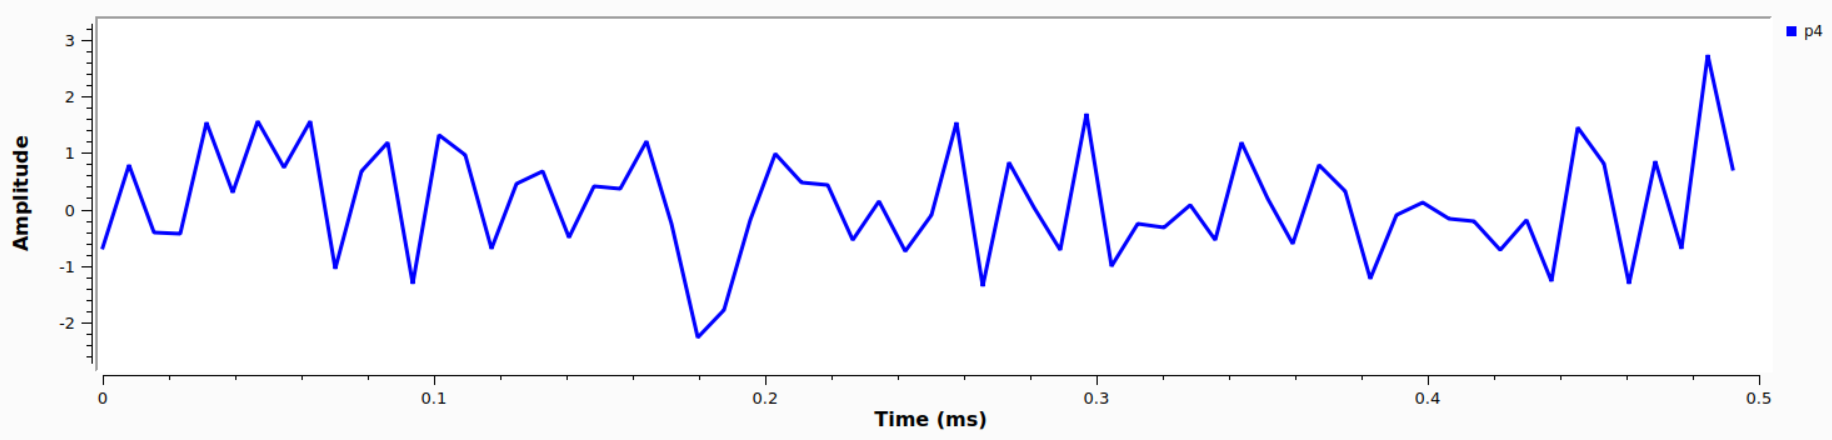
\includegraphics[width=\textwidth]{imagenes/ruido_puro_tiempo.png} 
    \caption{Ruido blanco en el dominio del tiempo.}
    \label{fig:ruido_tiempo}
\end{subfigure}
\hfill
\begin{subfigure}[b]{0.45\textwidth}
    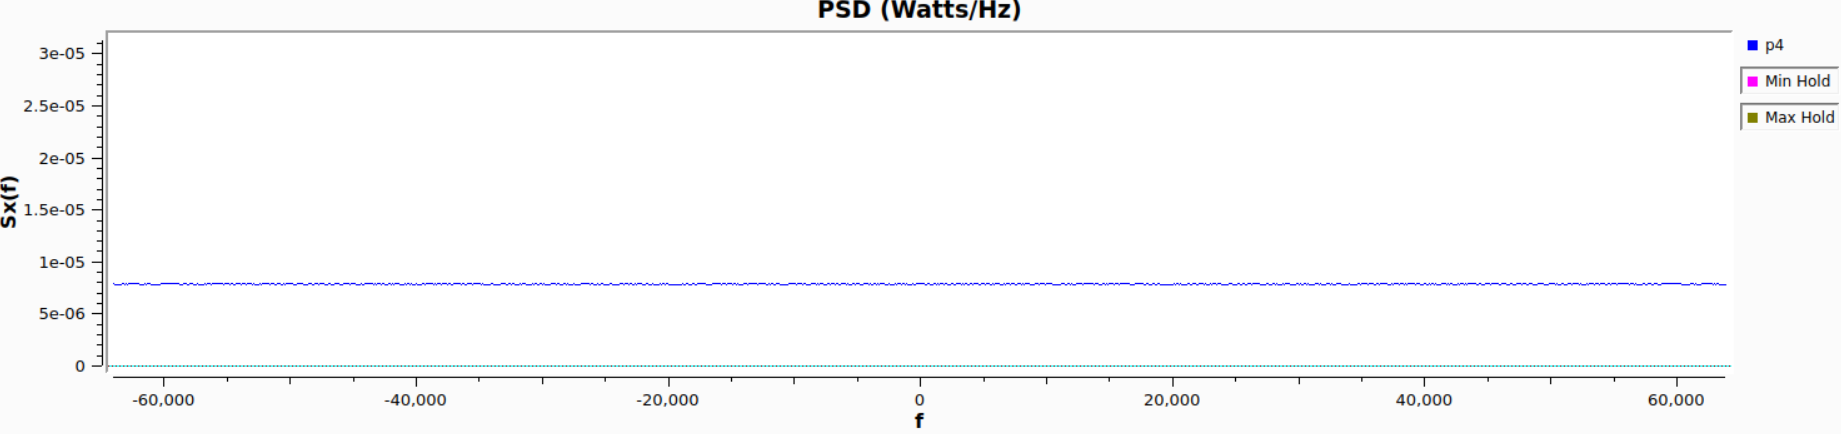
\includegraphics[width=\textwidth]{imagenes/ruido_puro_psd.png} 
    \caption{PSD del ruido blanco (Espectro plano).}
    \label{fig:ruido_psd}
\end{subfigure}
\caption{Análisis del ruido blanco gaussiano puro en los analizadores de GNU Radio.}
\label{fig:analisis_ruido_puro}
\end{figure}

\begin{figure}[htbp]
\centering
\begin{subfigure}[b]{0.45\textwidth}
    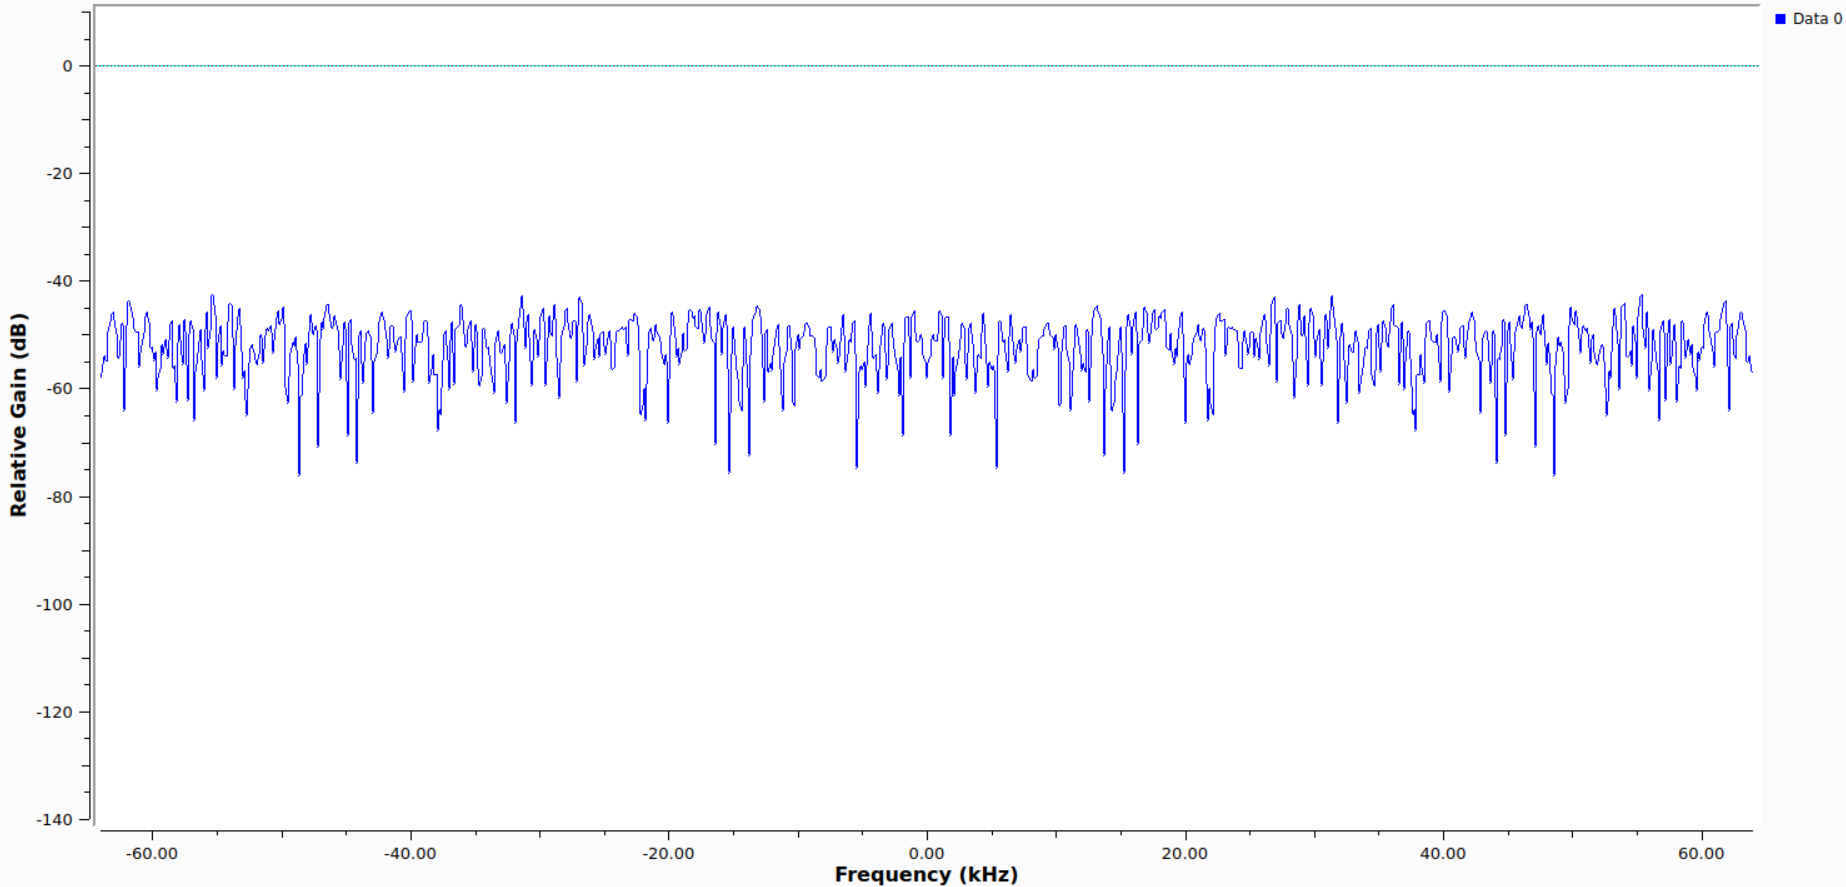
\includegraphics[width=\textwidth]{imagenes/espectro_amp_1.png} 
    \caption{espectro en frecuencia de ruido con amplitud de 1.}
    \label{fig:espectro_frecuencia_ruido_amp_1}
\end{subfigure}
\hfill
\begin{subfigure}[b]{0.45\textwidth}
    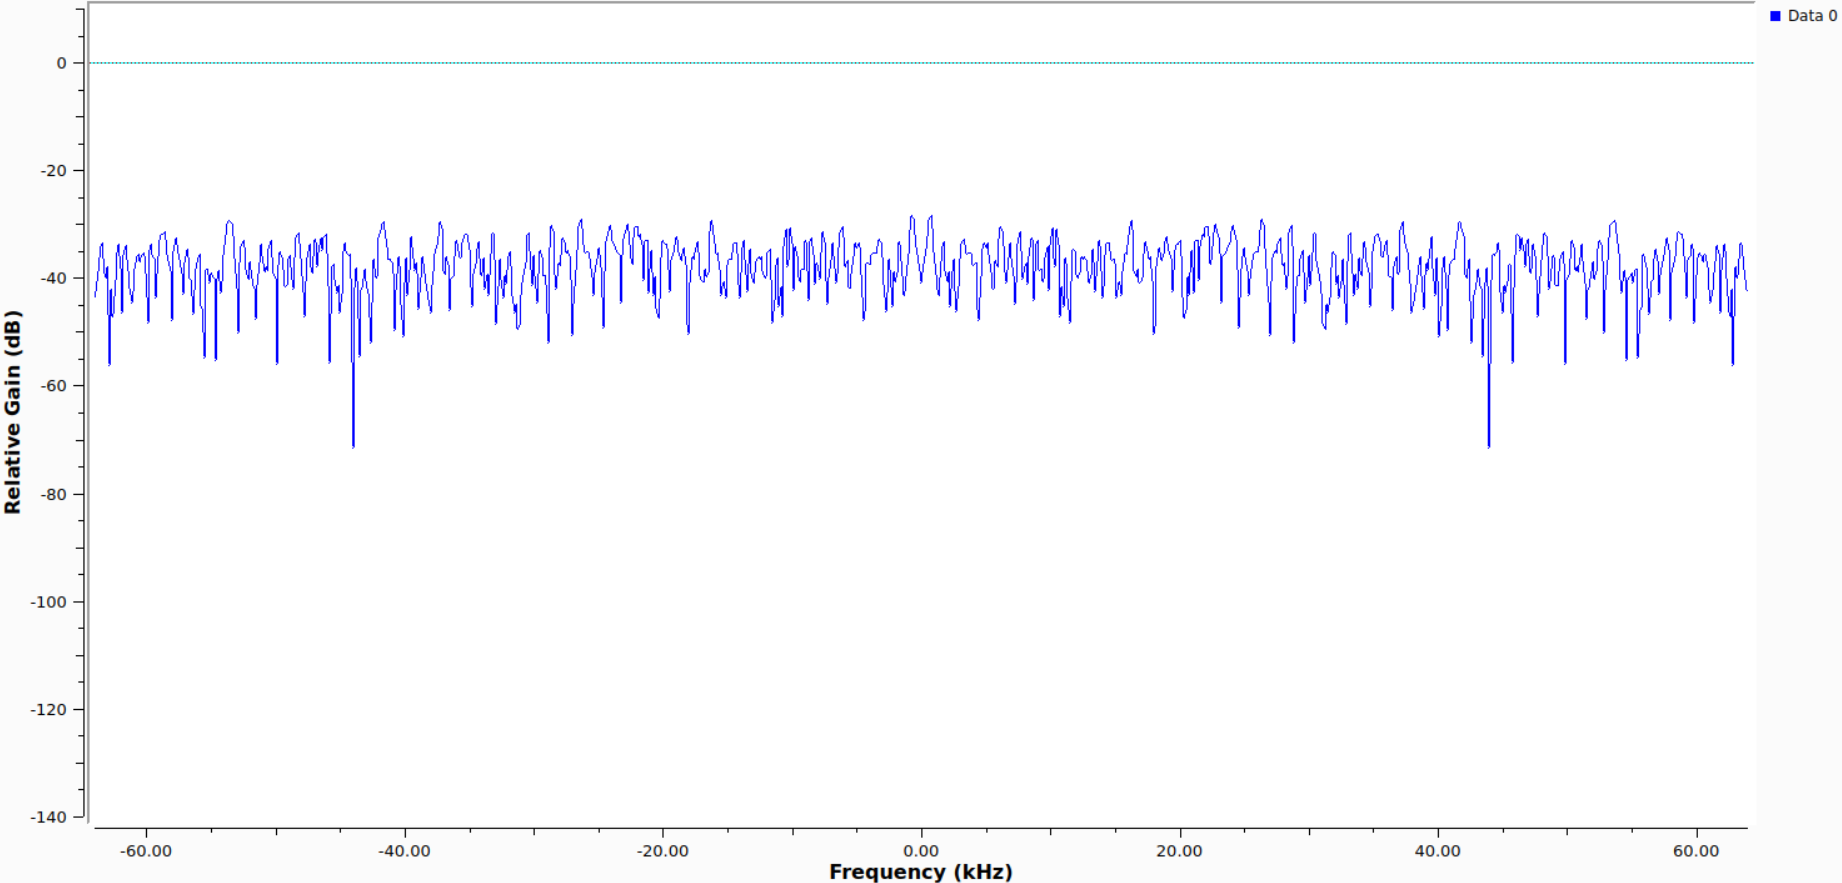
\includegraphics[width=\textwidth]{imagenes/espectro_amp_2.png} 
    \caption{espectro en frecuencia de ruido con amplitud de 0.2.}
    \label{fig:espectro_frecuencia_ruido_amp_0.2}
\end{subfigure}
\caption{cambio del nivel de potencia del ruido al variar la amplitud en el bloque generador.}
\label{fig:espectro_frecuencia_ruido}
\end{figure}
% --- FIN DEL MÓDULO ---
\subsection{Puntos 4 y 5: análisis con fuentes reales}

Para los puntos 4 y 5 se modificó el flujograma de la práctica con el fin de reemplazar la fuente binaria aleatoria por datos provenientes de archivos reales. En lugar del bloque \texttt{Random Source}, se utilizó una fuente de archivo cuyos bytes fueron descompuestos en bits para alimentar la misma cadena de procesamiento usada en la generación de la señal binaria rectangular. De esta manera, fue posible comparar el comportamiento temporal y espectral de una secuencia aleatoria ideal frente a secuencias obtenidas a partir de información del mundo real.

\subsubsection{Punto 4: archivo de imagen \texttt{rana}}

Para este caso se empleó como entrada el archivo \texttt{rana}. La señal obtenida en el dominio del tiempo se presenta en la Figura~\ref{fig:p4_tiempo_rana}. A diferencia de una fuente puramente aleatoria, aquí la secuencia presenta una estructura asociada al contenido del archivo, lo que se refleja en una distribución no completamente uniforme de transiciones entre niveles. En consecuencia, aunque la señal sigue siendo rectangular y binaria, su comportamiento estadístico ya no corresponde al de una fuente IID ideal.

\begin{figure}[H]
    \centering
    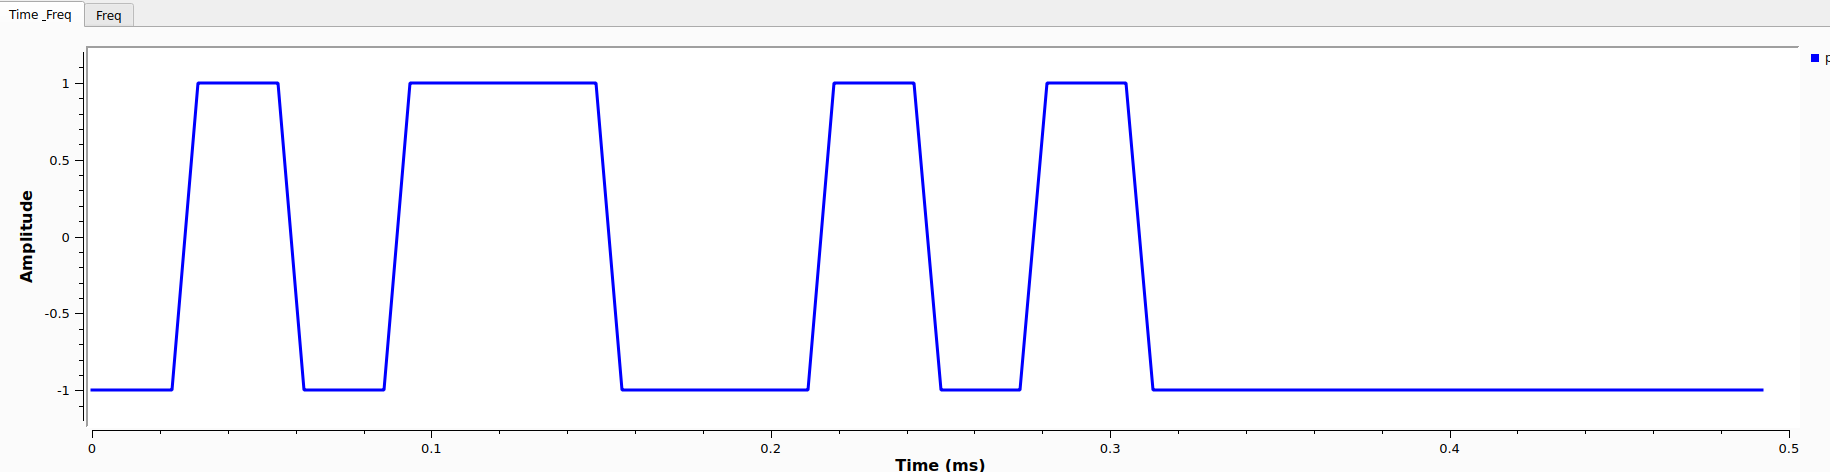
\includegraphics[width=0.86\linewidth]{imagenes/p4_tiempo_rana.png}
    \caption{Señal en el dominio del tiempo cuando la fuente de bits corresponde al archivo \texttt{rana}.}
    \label{fig:p4_tiempo_rana}
\end{figure}

La densidad espectral de potencia obtenida para esta señal se muestra en la Figura~\ref{fig:p4_psd_rana}. Se observa que la PSD conserva la envolvente general esperada para una señal binaria rectangular, pero su distribución energética no coincide exactamente con la de una fuente aleatoria ideal. Esto se debe a que los bits extraídos de una imagen real contienen redundancia y correlación, por lo que la energía no se reparte de forma completamente homogénea en frecuencia.

\begin{figure}[H]
    \centering
    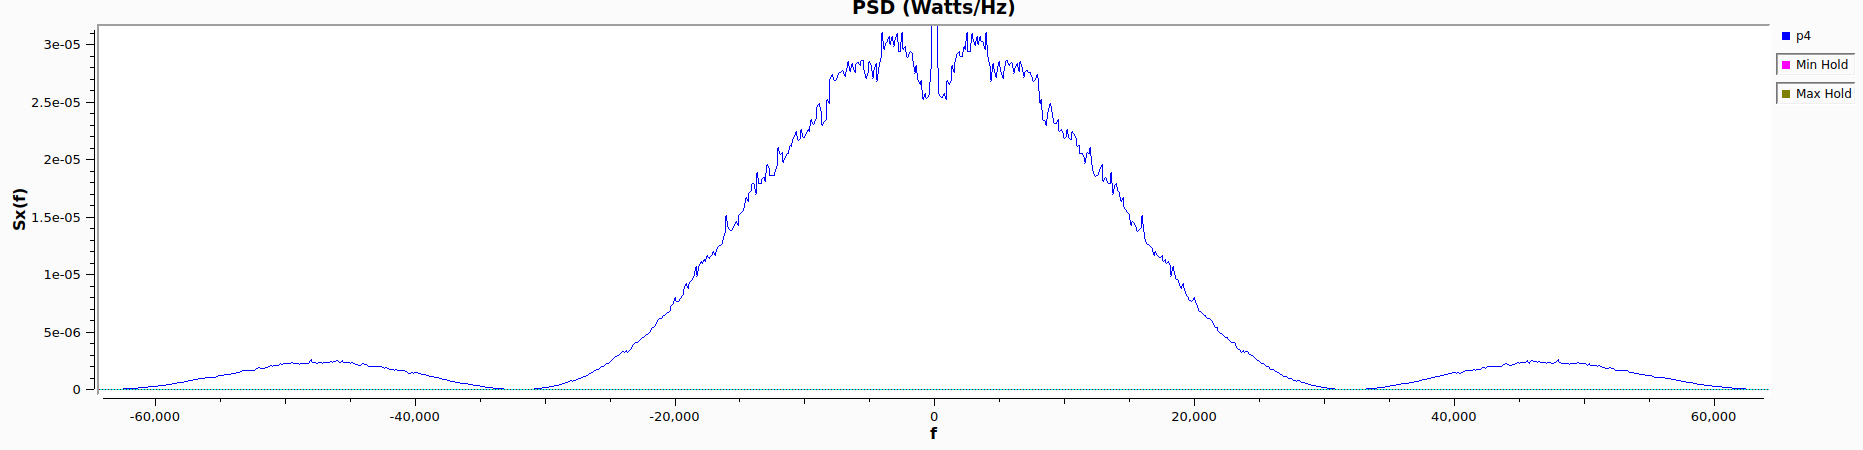
\includegraphics[width=0.86\linewidth]{imagenes/p4_psd_rana.png}
    \caption{PSD de la señal generada a partir del archivo \texttt{rana}.}
    \label{fig:p4_psd_rana}
\end{figure}

\subsubsection{Punto 5: archivo de audio \texttt{sonido}}

En el punto 5 se repitió el procedimiento anterior, pero utilizando el archivo \texttt{sonido} como fuente de datos. La señal temporal resultante se presenta en la Figura~\ref{fig:p5_tiempo_sonido}. En este caso también se conserva la forma rectangular de la señal, pero el patrón temporal observado responde a la estructura interna del audio digitalizado. Debido a la naturaleza del archivo, la secuencia de bits presenta una dependencia distinta a la de la imagen, lo cual modifica la estadística global de la señal.

\begin{figure}[H]
    \centering
    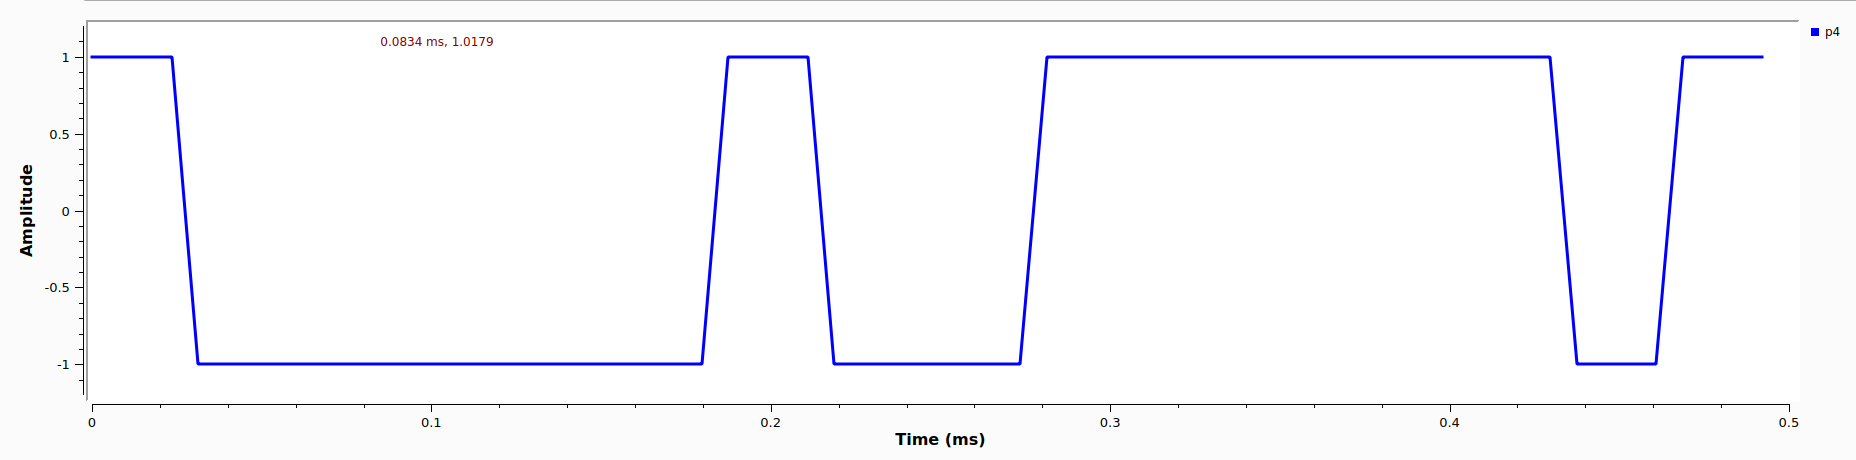
\includegraphics[width=0.86\linewidth]{imagenes/p5_tiempo_sonido.png}
    \caption{Señal en el dominio del tiempo cuando la fuente de bits corresponde al archivo \texttt{sonido}.}
    \label{fig:p5_tiempo_sonido}
\end{figure}

La PSD correspondiente se muestra en la Figura~\ref{fig:p5_psd_sonido}. Al compararla con la obtenida para el archivo de imagen, se evidencia que la forma espectral no es idéntica, aun cuando ambas señales se construyen finalmente como trenes rectangulares binarios. La diferencia se explica porque la fuente binaria ya no es aleatoria ideal, sino que depende del tipo de información almacenada en el archivo. En particular, los datos de audio suelen conservar cierta continuidad o correlación temporal entre muestras, lo cual influye en la distribución de energía del espectro.

\begin{figure}[H]
    \centering
    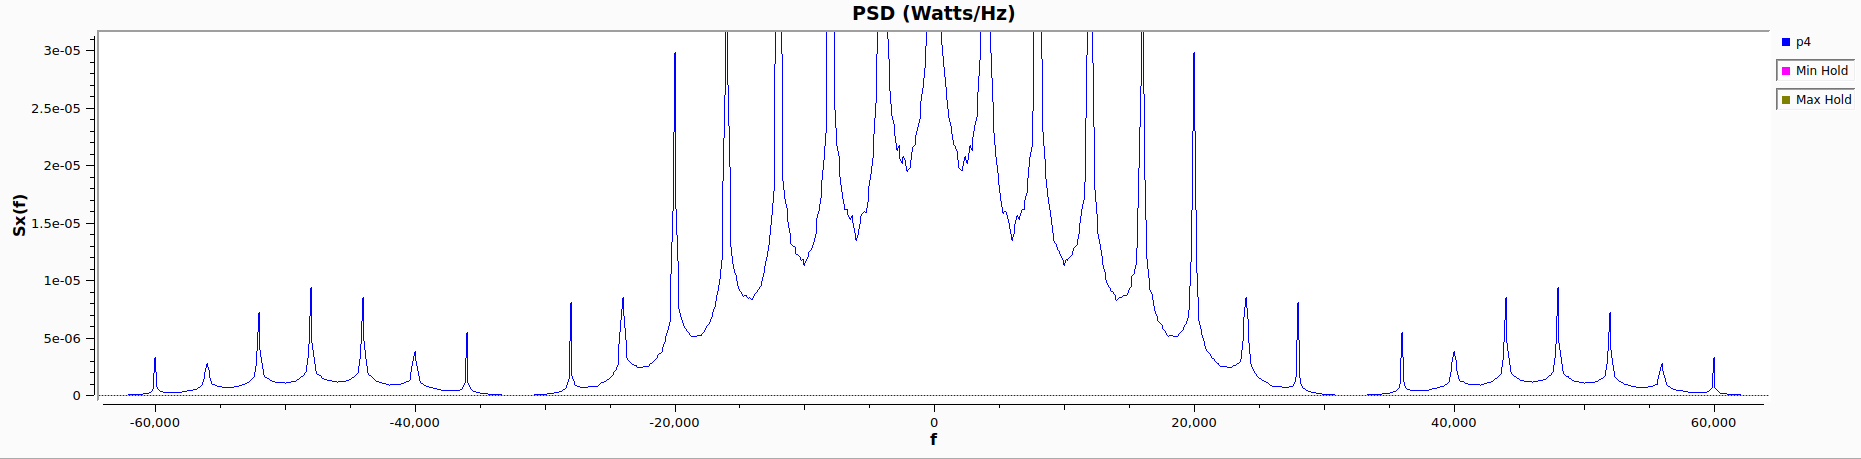
\includegraphics[width=0.86\linewidth]{imagenes/p5_psd_sonido.png}
    \caption{PSD de la señal generada a partir del archivo \texttt{sonido}.}
    \label{fig:p5_psd_sonido}
\end{figure}

\subsubsection{Caso complementario: efecto de aumentar \texttt{Sps} en la fuente de audio}

Como caso adicional, se analizó nuevamente la fuente \texttt{sonido} aumentando el número de muestras por símbolo a \(Sps=16\). La PSD obtenida se presenta en la Figura~\ref{fig:p5_psd_sonido_sps16}. Al incrementar \(Sps\), aumenta la frecuencia de muestreo de la señal rectangular, por lo que el espectro visible se extiende en un rango mayor de frecuencias. Sin embargo, la naturaleza espectral de la fuente no cambia: la señal sigue reflejando la estructura estadística propia del archivo de audio. Por tanto, variar \(Sps\) modifica la escala espectral y la forma en que se visualiza la PSD, pero no elimina la diferencia fundamental entre una fuente aleatoria ideal y una fuente real.

\begin{figure}[H]
    \centering
    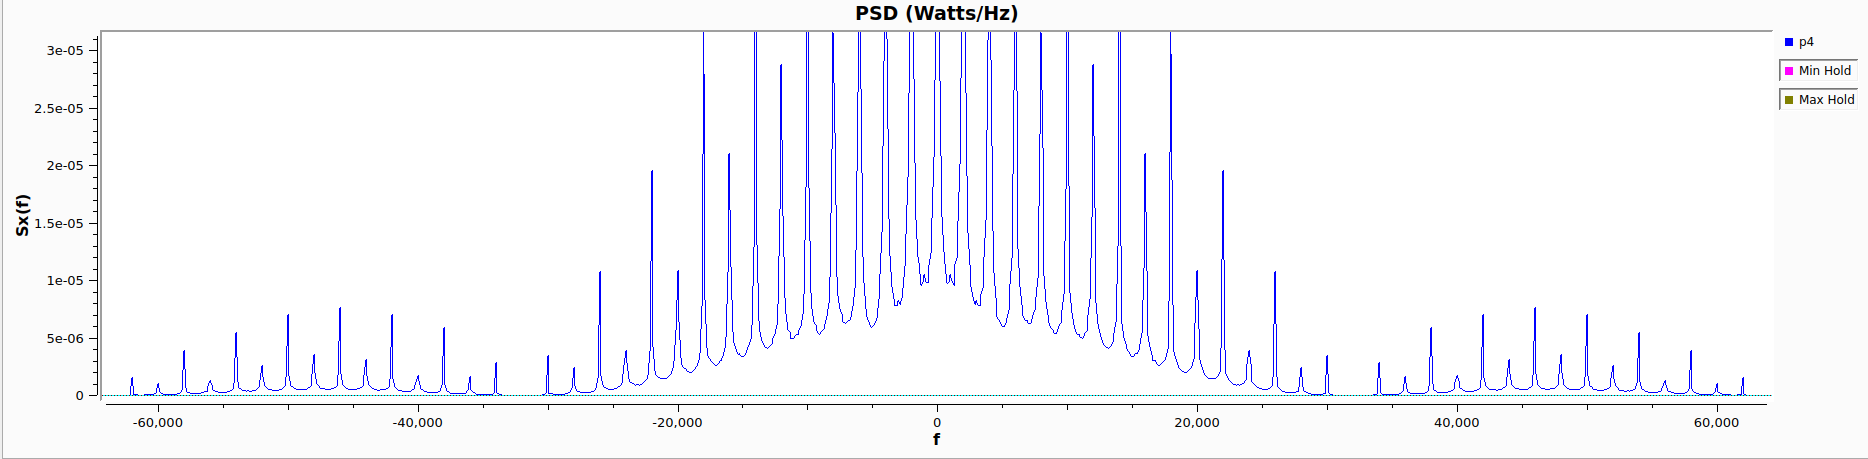
\includegraphics[width=0.86\linewidth]{imagenes/p5_psd_sonido_sps16.png}
    \caption{PSD de la señal obtenida a partir del archivo \texttt{sonido} usando \(Sps=16\).}
    \label{fig:p5_psd_sonido_sps16}
\end{figure}

En conjunto, los resultados de los puntos 4 y 5 muestran que la procedencia de los bits afecta de forma directa la apariencia temporal y espectral de la señal. Aunque en todos los casos la salida final corresponde a una señal binaria rectangular, el contenido estadístico de la fuente determina cómo se distribuye la energía en frecuencia. Por ello, una imagen y un audio, aun siendo almacenados digitalmente, no producen exactamente la misma PSD ni se comportan como una fuente binaria aleatoria ideal.
\subsection{Análisis del comportamiento espectral (Respuestas a–h)}

El procesamiento de la señal binaria en GNU Radio inicia con la conversión de una señal unipolar (0,1) a una señal bipolar (-1,1) mediante los bloques \textit{Constant Source}, \textit{Add} y \textit{Multiply Const}. Este proceso introduce un desplazamiento, centra la señal alrededor de cero y ajusta su amplitud, permitiendo eliminar el componente DC y obtener una PSD más simétrica.

El bloque \textit{Interpolation FIR Filter} realiza el sobremuestreo de la señal aumentando el número de muestras por símbolo (Sps), insertando muestras intermedias y aplicando un filtrado que suaviza la forma de los pulsos. El parámetro \textit{Interpolation} define este factor y debe coincidir con Sps para mantener coherencia entre la tasa de bits y la frecuencia de muestreo, evitando distorsiones en la señal y en su espectro. En este contexto, se cumple que:

\[
F_s = R_b \cdot Sps
\]

Para analizar la señal antes del sobremuestreo (p3), es necesario ubicar los instrumentos antes del bloque de interpolación y ajustar su frecuencia de muestreo. Además, el ancho de banda de la señal no depende de Sps, sino de la tasa de bits, por lo que se aproxima como:

\[
BW \approx 2 \cdot R_b
\]

Desde el punto de vista espectral, la PSD no solo depende de la forma del pulso, sino también de la naturaleza de la información. Señales provenientes de audio presentan mayor correlación entre bits y concentran su energía en bajas frecuencias, mientras que señales de imagen son más aleatorias y generan una PSD más uniforme.

El bloque \textit{Throttle} no modifica la señal, sino que controla la velocidad de procesamiento, evitando el uso excesivo de recursos y permitiendo una correcta visualización.

Si la señal no se convierte a bipolar y permanece en niveles 0 y 1, aparece un componente DC que genera un pico en frecuencia cero y una PSD no simétrica. Por otra parte, aunque teóricamente el ruido blanco y las señales rectangulares tienen ancho de banda infinito, en GNU Radio esto no se observa debido a la frecuencia de muestreo finita, que limita el espectro al rango de Nyquist:

\[
\pm \frac{F_s}{2}
\]

Finalmente, el número de lóbulos en la PSD está relacionado con el número de muestras por símbolo, cumpliéndose que:

\[
\text{Número de lóbulos} \approx Sps
\]

lo que indica que el sobremuestreo mejora la resolución espectral sin alterar el contenido fundamental de la señal.
\subsection{Ensayo técnico: análisis de las preguntas i--n}

El análisis de la PSD en GNU Radio permite relacionar directamente la tasa de bits, la frecuencia de muestreo y las operaciones internas del flujograma con la forma observable del espectro. Si la señal binaria rectangular tiene una tasa de bits \(R_b\) y el sistema utiliza \(Sps\) muestras por símbolo, entonces la frecuencia de muestreo en el punto donde ya se ha realizado la interpolación es

\[
f_s = R_b \cdot Sps.
\]

Como el analizador de espectros representa el eje frecuencial de forma simétrica alrededor del cero, el rango total de frecuencias ocupado por la visualización de la PSD es

\[
\left[-\frac{f_s}{2},\frac{f_s}{2}\right]
=
\left[-\frac{R_b Sps}{2},\frac{R_b Sps}{2}\right].
\]

De esta manera se responde cómo calcular todo el rango de frecuencias cuando se conocen \(R_b\) y \(Sps\).

La resolución espectral del analizador depende del número de puntos de la FFT y de la frecuencia de muestreo. Si el bloque utiliza una FFT de \(N\) puntos, la separación entre líneas espectrales consecutivas es

\[
\Delta f = \frac{f_s}{N}.
\]

Esto significa que un mayor número de puntos en la FFT mejora la resolución en frecuencia, mientras que una frecuencia de muestreo más alta aumenta el rango visible del espectro para un mismo valor de \(N\).

En cuanto al bloque \texttt{Unpack K Bits}, su función es convertir cada muestra de entrada en \(K\) bits de salida. Si la entrada corresponde a bytes de un archivo, el valor natural es \(K=8\), puesto que cada byte contiene ocho bits. Si se configurara \(K=16\), la tasa de salida del bloque se duplicaría con respecto al caso normal, es decir,

\[
f_{s,\text{out}}^{(\text{Unpack})} = K\,f_{s,\text{in}}^{(\text{Unpack})},
\]

pero además se perdería coherencia con la estructura original del archivo, ya que se estaría forzando una descomposición de 16 bits sobre datos almacenados de manera natural en palabras de 8 bits. En la práctica, esto alteraría la interpretación correcta de la información y modificaría artificialmente la velocidad del flujo de datos.

Si se conoce el número de lóbulos observados en la PSD y el ancho de banda característico asociado a cada lóbulo, puede estimarse primero la frecuencia de muestreo visible en el analizador. Si se denota por \(L\) el número de lóbulos contados según la convención del laboratorio y por \(B\) el ancho asociado a cada lóbulo, entonces una aproximación útil es

\[
f_{s,\text{PSD}} \approx L \, B.
\]

Una vez obtenida esa frecuencia de muestreo en el punto de observación, es posible retroceder por el flujograma para hallar la frecuencia a la entrada del bloque \texttt{Unpack K Bits}. Si la señal observada ya pasó por el \texttt{Unpack K Bits} y luego por una interpolación de factor \(Sps\), entonces

\[
f_{s,\text{in}}^{(\text{Unpack})}
=
\frac{f_{s,\text{PSD}}}{K \cdot Sps}.
\]

A partir de esta expresión se deduce también la frecuencia de muestreo a la salida del propio bloque \texttt{Unpack K Bits}, que simplemente queda dada por

\[
f_{s,\text{out}}^{(\text{Unpack})}
=
K\,f_{s,\text{in}}^{(\text{Unpack})}.
\]

Por su parte, el bloque \texttt{Char to Float} no cambia la tasa de muestreo. Su función es únicamente convertir el tipo de dato para que las muestras puedan ser procesadas en formato numérico de punto flotante por los bloques siguientes. Por ello, si se conoce la frecuencia de muestreo a su entrada, la frecuencia a su salida permanece igual:

\[
f_{s,\text{out}}^{(\text{Char to Float})}
=
f_{s,\text{in}}^{(\text{Char to Float})}.
\]

En síntesis, el rango frecuencial visible en la PSD lo fija la frecuencia de muestreo, la resolución del analizador depende de la FFT, el bloque \texttt{Unpack K Bits} multiplica la tasa por \(K\), y el bloque \texttt{Char to Float} conserva dicha tasa. Estas relaciones permiten interpretar correctamente el comportamiento del espectro observado en GNU Radio y justifican matemáticamente los cambios producidos al modificar la fuente de datos o los parámetros del flujograma.
% --- INICIO DEL MÓDULO SINTETIZADO: 05_preguntas_o_x.tex ---

\subsection{Conformación de Pulso, Códigos de Línea y Modulación (6.o - 6.x)}

La alteración paramétrica del filtro interpolador $h$ y las Muestras por Símbolo ($Sps$) permite adaptar la señal a las restricciones del canal. En el límite teórico ($Sps=1$), la señal pierde su envolvente temporal, convirtiéndose en muestras aleatorias descorrelacionadas cuyo espectro es plano, equivalente a ruido blanco discreto (6.o). Al restaurar un $Sps=4$, se evaluaron diferentes geometrías de pulso. El uso de una rampa asimétrica o Diente de Sierra ($h=[0.25, 0.5, 0.75, 1]$) (6.p) genera transiciones abruptas que degradan la atenuación de los lóbulos laterales en la Densidad Espectral de Potencia (PSD), incrementando la interferencia de canal adyacente. Por otro lado, el formato RZ ($h=[1, 1, 0, 0]$) (6.q) retorna a cero a mitad del símbolo; esta compresión temporal duplica el consumo de ancho de banda ($2R_b$). En contraste, el código Manchester ($h=[1, 1, -1, -1]$) (6.r) fuerza una transición interna que equilibra el área de voltaje a cero. Esto elimina por completo el impulso ineficiente de Corriente Continua en $0\text{ Hz}$, demostrando la superioridad energética de los formatos bipolares balanceados frente a los unipolares (6.x).

Para trasladar la información a radiofrecuencia (paso-banda), se inyectaron arreglos senoidales (\texttt{np.sin}) en el filtro. Las modulaciones de amplitud como OOK y ASK (6.s, 6.u) desplazan el espectro, pero desperdician potencia al transmitir una portadora pura. Sin embargo, al mantener datos de entrada bipolares, se logra la modulación BPSK (6.t). En este esquema, los bits negativos invierten matemáticamente la senoide, generando saltos de fase de $180^\circ$ que suprimen la portadora central en la PSD, maximizando la eficiencia de transmisión.

Finalmente, para la mitigación de la Interferencia Intersimbólica (ISI), se implementaron pulsos tipo sinc (6.v) y filtros de Raíz de Coseno Alzado (6.w). El uso de la función \texttt{firdes.root\_raised\_cosine} demostró ser el esquema de mayor eficiencia espectral: sus oscilaciones temporales amortiguadas ("pulsos rizados") logran anular de forma absoluta los lóbulos laterales en la frecuencia, confinando la energía de la señal en un bloque libre de fugas espectrales.

% --- FIGURA DE SÍNTESIS (3 SUBFIGURAS CLAVE) ---
\begin{figure}[htbp]
\centering
\begin{subfigure}[b]{0.5\textwidth}
    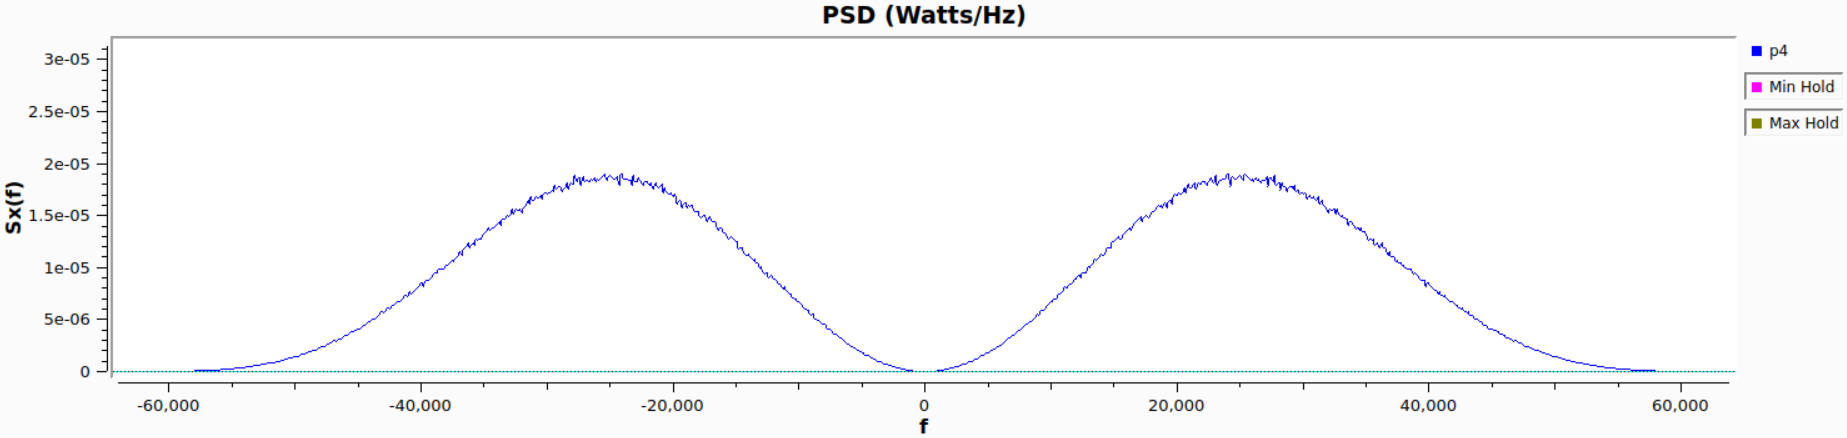
\includegraphics[width=\textwidth]{imagenes/captura_manchester.png} % Usa tu captura de la PSD de Manchester
    \caption{PSD Manchester: Eliminación de la componente DC.}
    \label{fig:sintesis_manchester}
\end{subfigure}
\hfill
\begin{subfigure}[b]{0.5\textwidth}
    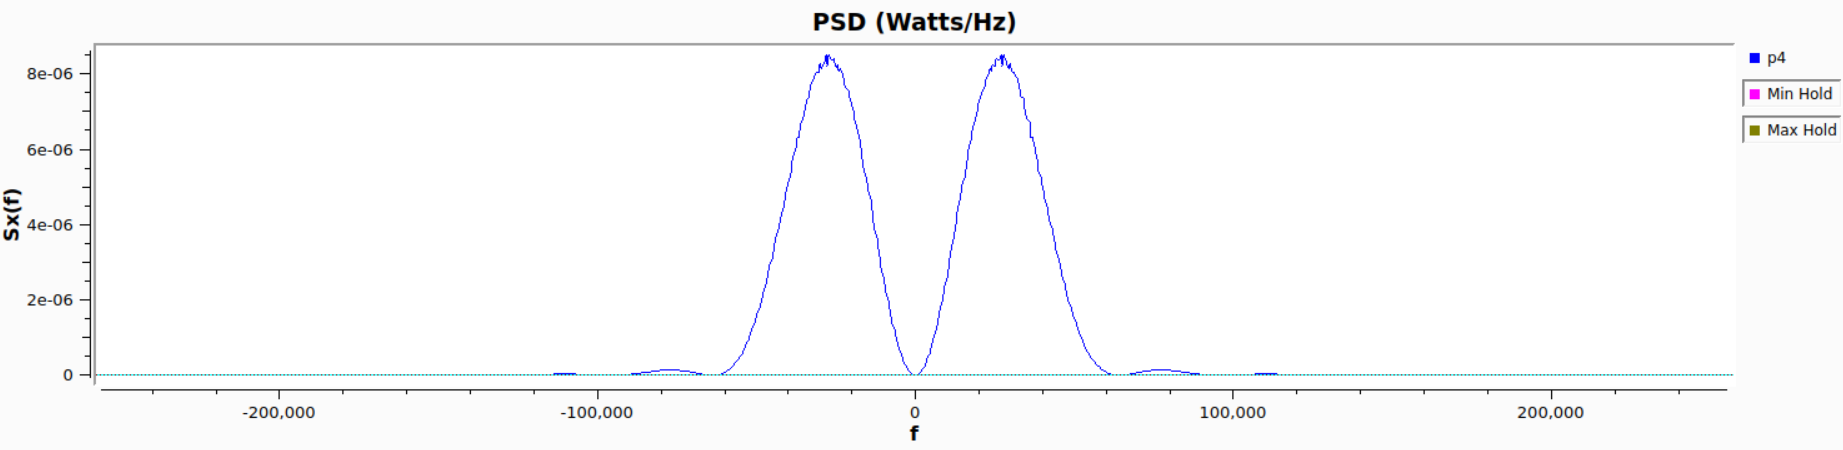
\includegraphics[width=\textwidth]{imagenes/captura_bpsk.png} % Usa tu captura del tiempo (osciloscopio) de BPSK
    \caption{BPSK (Tiempo): Saltos de fase de $180^\circ$.}
    \label{fig:sintesis_bpsk}
\end{subfigure}
\hfill
\begin{subfigure}[b]{0.5\textwidth}
    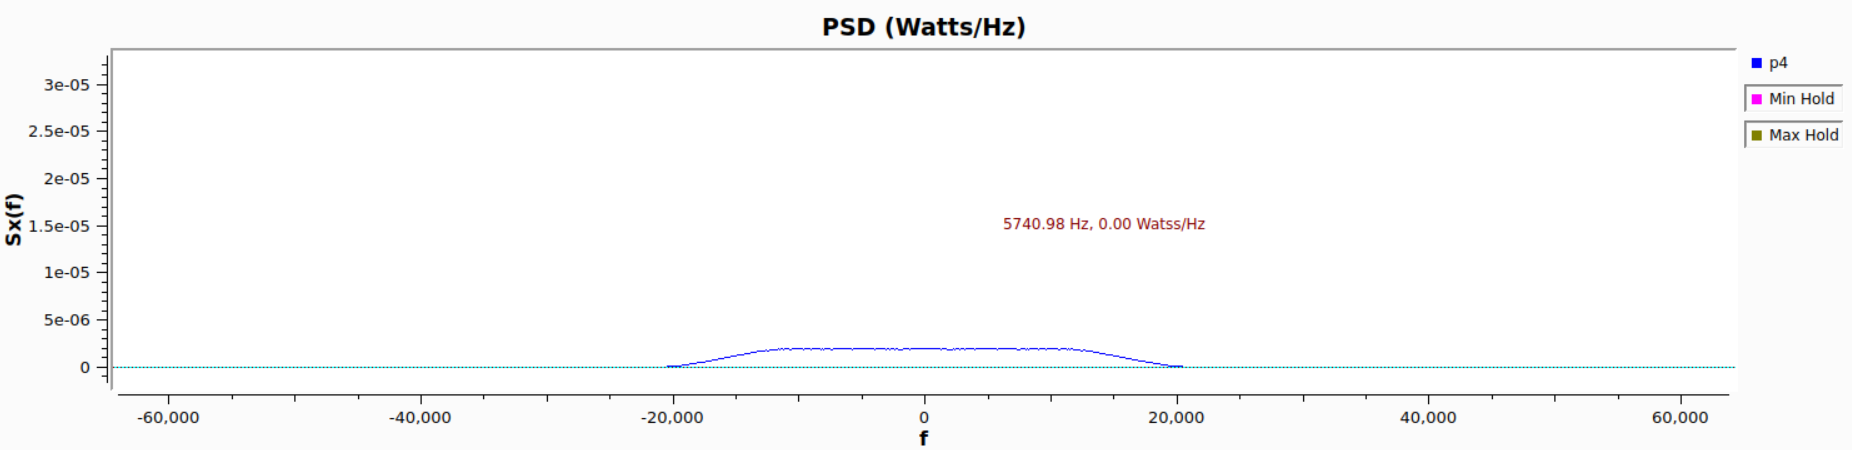
\includegraphics[width=\textwidth]{imagenes/captura_coseno.png} % Usa tu captura de la PSD del Coseno Alzado
    \caption{PSD Coseno Alzado: Supresión de lóbulos laterales.}
    \label{fig:sintesis_coseno}
\end{subfigure}
\caption{Análisis comparativo de las técnicas de codificación, modulación y conformación de pulso más relevantes.}
\label{fig:sintesis_total}
\end{figure}
% --- FIN DEL MÓDULO SINTETIZADO ---





% --- INICIO DEL MÓDULO: 04_conclusiones.tex ---

\section{Conclusiones}

El incremento de \(Sps\) mejora la representación temporal de la señal y permite observar con mayor claridad la estructura de la PSD, sin modificar el ancho de banda fundamental determinado por la tasa de bits.


Las señales obtenidas a partir de \texttt{rana.jpg} y \texttt{sonido.wav} presentan distribuciones espectrales distintas a las de una fuente binaria aleatoria ideal, debido a la correlación estadística propia de cada archivo.


Las modificaciones realizadas sobre el filtro interpolador mostraron que la codificación de línea y la conformación de pulso alteran la componente DC y la ocupación espectral de la señal, por lo que la elección del pulso influye directamente en la eficiencia de transmisión.

\begin{thebibliography}{99}

\bibitem{guia_lab3}
Escuela de Ingenierías Eléctrica, Electrónica y de Telecomunicaciones,
\textit{Guía de Laboratorio 3: PSD de Señales Aleatorias (GNU Radio)},
Comunicaciones II, Universidad Industrial de Santander.

\bibitem{ortega_reyes}
H. Ortega Boada y Ó. M. Reyes Torres,
\textit{Comunicaciones Digitales basadas en radio definida por software. Volumen I},
Bucaramanga, Colombia: Universidad Industrial de Santander.

\bibitem{proakis}
J. G. Proakis y M. Salehi,
\textit{Digital Communications},
5th ed., New York, NY, USA: McGraw-Hill, 2008.

\bibitem{couch}
L. W. Couch,
\textit{Digital and Analog Communication Systems},
8th ed., Upper Saddle River, NJ, USA: Pearson, 2013.

\bibitem{lathi}
B. P. Lathi y Z. Ding,
\textit{Modern Digital and Analog Communication Systems},
4th ed., New York, NY, USA: Oxford University Press, 2009.

\bibitem{gnuradio}
GNU Radio Project,
``GNU Radio: The Free \& Open Software Radio Ecosystem.''
[Online]. Available: \url{https://www.gnuradio.org/}

\end{thebibliography}
%\input{modulos/00_abstract}
%\input{modulos/01_introduccion}
%\input{modulos/02_metodologia}
%\input{modulos/03_resultados}
%\input{modulos/04_conclusiones}

% --- Referencias (Pueden ir aquí o en un módulo aparte) ---
\begin{thebibliography}{00}
\bibitem{b1} Escuela de Ingenierías Eléctrica, Electrónica y de Telecomunicaciones, \textit{Guía de Laboratorio 3: PSD de Señales Aleatorias (GNURadio)}, Comunicaciones II.
\end{thebibliography}

\end{document}